\documentclass[aspectratio=169, 9pt]{beamer}

% ==============================================================================
% THEME & NAVIGATION CONFIGURATION
% ==============================================================================
\usetheme[sectionpage=none]{metropolis}
\useoutertheme[subsection=false]{miniframes}
\nonstopmode

% ==============================================================================
% REQUIRED PACKAGES
% ==============================================================================
\usepackage{bookmark}
\usepackage{tikz}
\usetikzlibrary{shapes.geometric, arrows.meta, positioning, calc, shadows.blur}

\usepackage[utf8]{inputenc}
\usepackage[T1]{fontenc}
\usepackage{lmodern}
\usepackage{graphicx}
\graphicspath{{../assets/}{assets/}{templates/assets/}{../../templates/assets/}{./}}

\usepackage[backend=biber, style=numeric, sorting=none, maxnames=2, natbib=true, doi=false, url=false, isbn=false]{biblatex}
\addbibresource{references.bib}

\usepackage[most]{tcolorbox}
\usepackage{booktabs}
\usepackage{array}
\usepackage{colortbl}
\usepackage{listings}
\usepackage{amsmath, amssymb, amsfonts}

% ==============================================================================
% COLOR PALETTE (Editorial Crimson, Slate & Journal Navy)
% ==============================================================================
\definecolor{background}{RGB}{255, 255, 255}
\definecolor{foreground}{RGB}{30, 30, 40}
\definecolor{accent}{RGB}{220, 40, 40}
\definecolor{structure}{RGB}{50, 50, 60}
\definecolor{journalblue}{RGB}{26, 82, 118}
\definecolor{tableheader}{RGB}{240, 244, 248}

\setbeamercolor{normal text}{fg=foreground, bg=background}
\setbeamercolor{alerted text}{fg=accent}
\setbeamercolor{frametitle}{fg=foreground, bg=background}
\setbeamercolor{title separator}{fg=accent}
\setbeamercolor{section in head/foot}{fg=foreground, bg=structure!6}
\setbeamercolor{mini frame}{fg=accent, bg=structure!25}

\setbeamerfont{frametitle}{size=\large, series=\bfseries}
\setbeamerfont{title}{size=\Large, series=\bfseries}
\setbeamerfont{subtitle}{size=\normalsize}

% Progress Bar Header
\setbeamertemplate{headline}{%
  \begin{beamercolorbox}[wd=\paperwidth]{section in head/foot}
    \vskip3pt\centering
    \insertnavigation{0.7\paperwidth}%
    \vskip3pt%
  \end{beamercolorbox}%
  {\color{accent}\hrule height 2pt}%
}

% Minimalist Page Number Footer
\setbeamertemplate{footline}{%
  \vspace{3pt}%
  \hfill\usebeamercolor[fg]{page number in head/foot}\usebeamerfont{page number in head/foot}\insertframenumber\hspace*{1.2em}\vspace{3pt}%
}

% UI Helpers
\setbeamertemplate{itemize item}{\raisebox{0.18ex}{\textcolor{accent}{\rule{0.38em}{0.38em}}}}
\setbeamertemplate{itemize subitem}{\raisebox{0.15ex}{\textcolor{accent!60}{\rule{0.28em}{0.28em}}}}
\setlength{\labelsep}{0.5em}

\newtcbox{\pill}{on line, enhanced, colframe=accent, boxrule=0pt, arc=2.5pt,
  interior style={top color=accent, bottom color=accent!85},
  coltext=white, left=4pt, right=4pt, top=1.2pt, bottom=1.2pt,
  fontupper=\fontsize{6pt}{7pt}\selectfont\bfseries\sffamily}

\newtcbox{\pillalt}{on line, enhanced, colframe=structure, boxrule=0pt, arc=2.5pt,
  interior style={top color=structure!85, bottom color=structure!70},
  coltext=white, left=4pt, right=4pt, top=1.2pt, bottom=1.2pt,
  fontupper=\fontsize{6pt}{7pt}\selectfont\bfseries\sffamily}

\newtcolorbox{takeaway}[1][]{enhanced, colframe=accent, boxrule=0pt, leftrule=2.5pt,
  interior style={left color=accent!10, right color=accent!2},
  arc=1.5pt, outer arc=1.5pt, left=5pt, right=5pt, top=3pt, bottom=3pt,
  fontupper=\scriptsize, before skip=3pt, after skip=2pt, #1}

\newcommand{\kpicard}[3]{%
  \begin{tcolorbox}[enhanced, colframe=structure!20, colback=structure!3, boxrule=0.5pt, arc=2pt,
    left=3pt, right=3pt, top=2.5pt, bottom=2.5pt, halign=center]
    {\fontsize{6pt}{7pt}\selectfont\bfseries\textcolor{structure}{#1}}\\[1pt]
    {\normalsize\bfseries\textcolor{accent}{#2}}\\[1pt]
    {\tiny\textcolor{structure!70}{#3}}
  \end{tcolorbox}%
}

% ==============================================================================
% PRESENTATION METADATA
% ==============================================================================
\title{Econometric Identification and Causal Inference}
\subtitle{Panel Two-Way Fixed Effects, Difference-in-Differences, and Robust Covariance}
\author{Prof.~Elena Rostova \and Dr.~Alex Morgan}
\institute{Department of Economics \& Institute for Empirical Research}
\date{\today}

\setbeamertemplate{title page}{
  \vfill
  \centering
  
\includegraphics[height=1.3cm]{university_seal.jpg}\par\vspace{0.4em}
  \usebeamerfont{title}\inserttitle\par
  \vspace{0.2em}
  \usebeamerfont{subtitle}\textcolor{structure}{\insertsubtitle}\par
  \vspace{0.5em}
  {\color{accent}\rule{0.75\textwidth}{1.2pt}}\par
  \vspace{0.5em}
  \usebeamerfont{author}\insertauthor\par
  \vspace{0.2em}
  \usebeamerfont{institute}\textcolor{structure!75}{\insertinstitute}\par
  \vspace{0.2em}
  \usebeamerfont{date}\textcolor{structure!55}{\insertdate}\par
  \vfill
}

% ==============================================================================
% DOCUMENT BEGIN
% ==============================================================================
\begin{document}

% --- Slide 1: Title ---
\begin{frame}[plain]
    \titlepage
\end{frame}

% --- Slide 2: Roadmap ---
\section{Roadmap}
\begin{frame}{Econometric Roadmap \& Methodological Pillars}
    \begin{columns}[c]
        \begin{column}{0.48\textwidth}
            \pillalt{ROADMAP}\par\vspace{0.3em}
            \begin{itemize}\setlength{\itemsep}{2.5pt}
                \item \textbf{1. Causal Potential Outcomes:} SUTVA and unconfoundedness~\cite{angrist1996identification}.
                \item \textbf{2. Panel Data \& TWFE:} Within transformation eliminating individual heterogeneity.
                \item \textbf{3. Difference-in-Differences:} Parallel trends and counterfactual simulations~\cite{callaway2021difference}.
                \item \textbf{4. Robust Covariance:} Liang-Zeger cluster corrections~\cite{wooldridge2010econometric}.
                \item \textbf{5. Empirical Estimation:} Multi-specification regression tables.
            \end{itemize}
        \end{column}
        \begin{column}{0.48\textwidth}
            \begin{takeaway}
                \textbf{\textcolor{accent}{Identification Invariant:}} Causal parameters are identified only when unobserved confounders are absorbed by quasi-experimental variation.
            \end{takeaway}
            \vspace{0.4em}
            \begin{columns}[c]
                \begin{column}{0.48\textwidth}
                    \kpicard{PANEL SAMPLE}{$N = 45{,}200$}{Longitudinal Units}
                \end{column}
                \begin{column}{0.48\textwidth}
                    \kpicard{CLUSTERS}{$G = 120$}{Independent Groups}
                \end{column}
            \end{columns}
        \end{column}
    \end{columns}
\end{frame}

% --- Slide 3: Two-Way Fixed Effects ---
\section{Panel}
\begin{frame}{Panel Data: Two-Way Fixed Effects (TWFE)}
    \begin{columns}[t]
        \begin{column}{0.48\textwidth}
            \pillalt{PANEL SPECIFICATION}\par\vspace{0.2em}
            \scriptsize
            Standard linear two-way fixed effects model:
            \begin{equation*}
                Y_{it} = \alpha_i + \lambda_t + \delta D_{it} + \mathbf{X}_{it}^\top \boldsymbol{\beta} + \varepsilon_{it}
            \end{equation*}
            \vspace{0.1em}
            \begin{itemize}\setlength{\itemsep}{2pt}
                \item \textbf{Unit Heterogeneity ($\alpha_i$):} Time-invariant unobservables.
                \item \textbf{Time Shocks ($\lambda_t$):} Common macroeconomic trends.
                \item \textbf{Treatment ($D_{it}$):} Binary policy exposure indicator.
            \end{itemize}
        \end{column}
        \begin{column}{0.48\textwidth}
            \pill{WITHIN DEMEANING}\par\vspace{0.2em}
            \scriptsize
            Applying the within transformation eliminates $\alpha_i$:
            \begin{equation*}
                \ddot{Y}_{it} = \delta \ddot{D}_{it} + \ddot{\mathbf{X}}_{it}^\top \boldsymbol{\beta} + \ddot{\varepsilon}_{it}
            \end{equation*}
            where $\ddot{Y}_{it} = Y_{it} - \bar{Y}_i - \bar{Y}_t + \bar{Y}$.
            \vspace{0.2em}
            \begin{takeaway}
                \textbf{Gauss-Markov Condition:} Strict exogeneity $\mathbb{E}[\varepsilon_{it} \mid \mathbf{X}_i, \mathbf{D}_i, \alpha_i] = 0$ guarantees unbiasedness $\mathbb{E}[\hat{\delta}_{\mathrm{FE}}] = \delta$.
            \end{takeaway}
        \end{column}
    \end{columns}
\end{frame}

% --- Slide 4: Difference-in-Differences Simulation ---
\section{DiD}
\begin{frame}{Causal Estimation: Difference-in-Differences}
    \begin{columns}[c]
        \begin{column}{0.44\textwidth}
            \pillalt{DID ESTIMATOR}\par\vspace{0.2em}
            \scriptsize
            Canonical $2 \times 2$ formulation:
            \begin{equation*}
                \hat{\delta}_{\mathrm{DiD}} = (\bar{Y}_{T,2} - \bar{Y}_{T,1}) - (\bar{Y}_{C,2} - \bar{Y}_{C,1})
            \end{equation*}
            \vspace{0.1em}
            \begin{itemize}\setlength{\itemsep}{1.5pt}
                \item \textbf{Parallel Trends Invariant:}
                $\mathbb{E}[\Delta Y_i(0) \mid D_i=1] = \mathbb{E}[\Delta Y_i(0) \mid D_i=0]$.
                \item \textbf{Counterfactual:} Expected trajectory of treated units absent the reform.
                \item \textbf{Empirical Effect:} $\hat{\delta} = +3.60^{***}$ ($p < 0.001$).
            \end{itemize}
        \end{column}
        \begin{column}{0.54\textwidth}
            \centering
            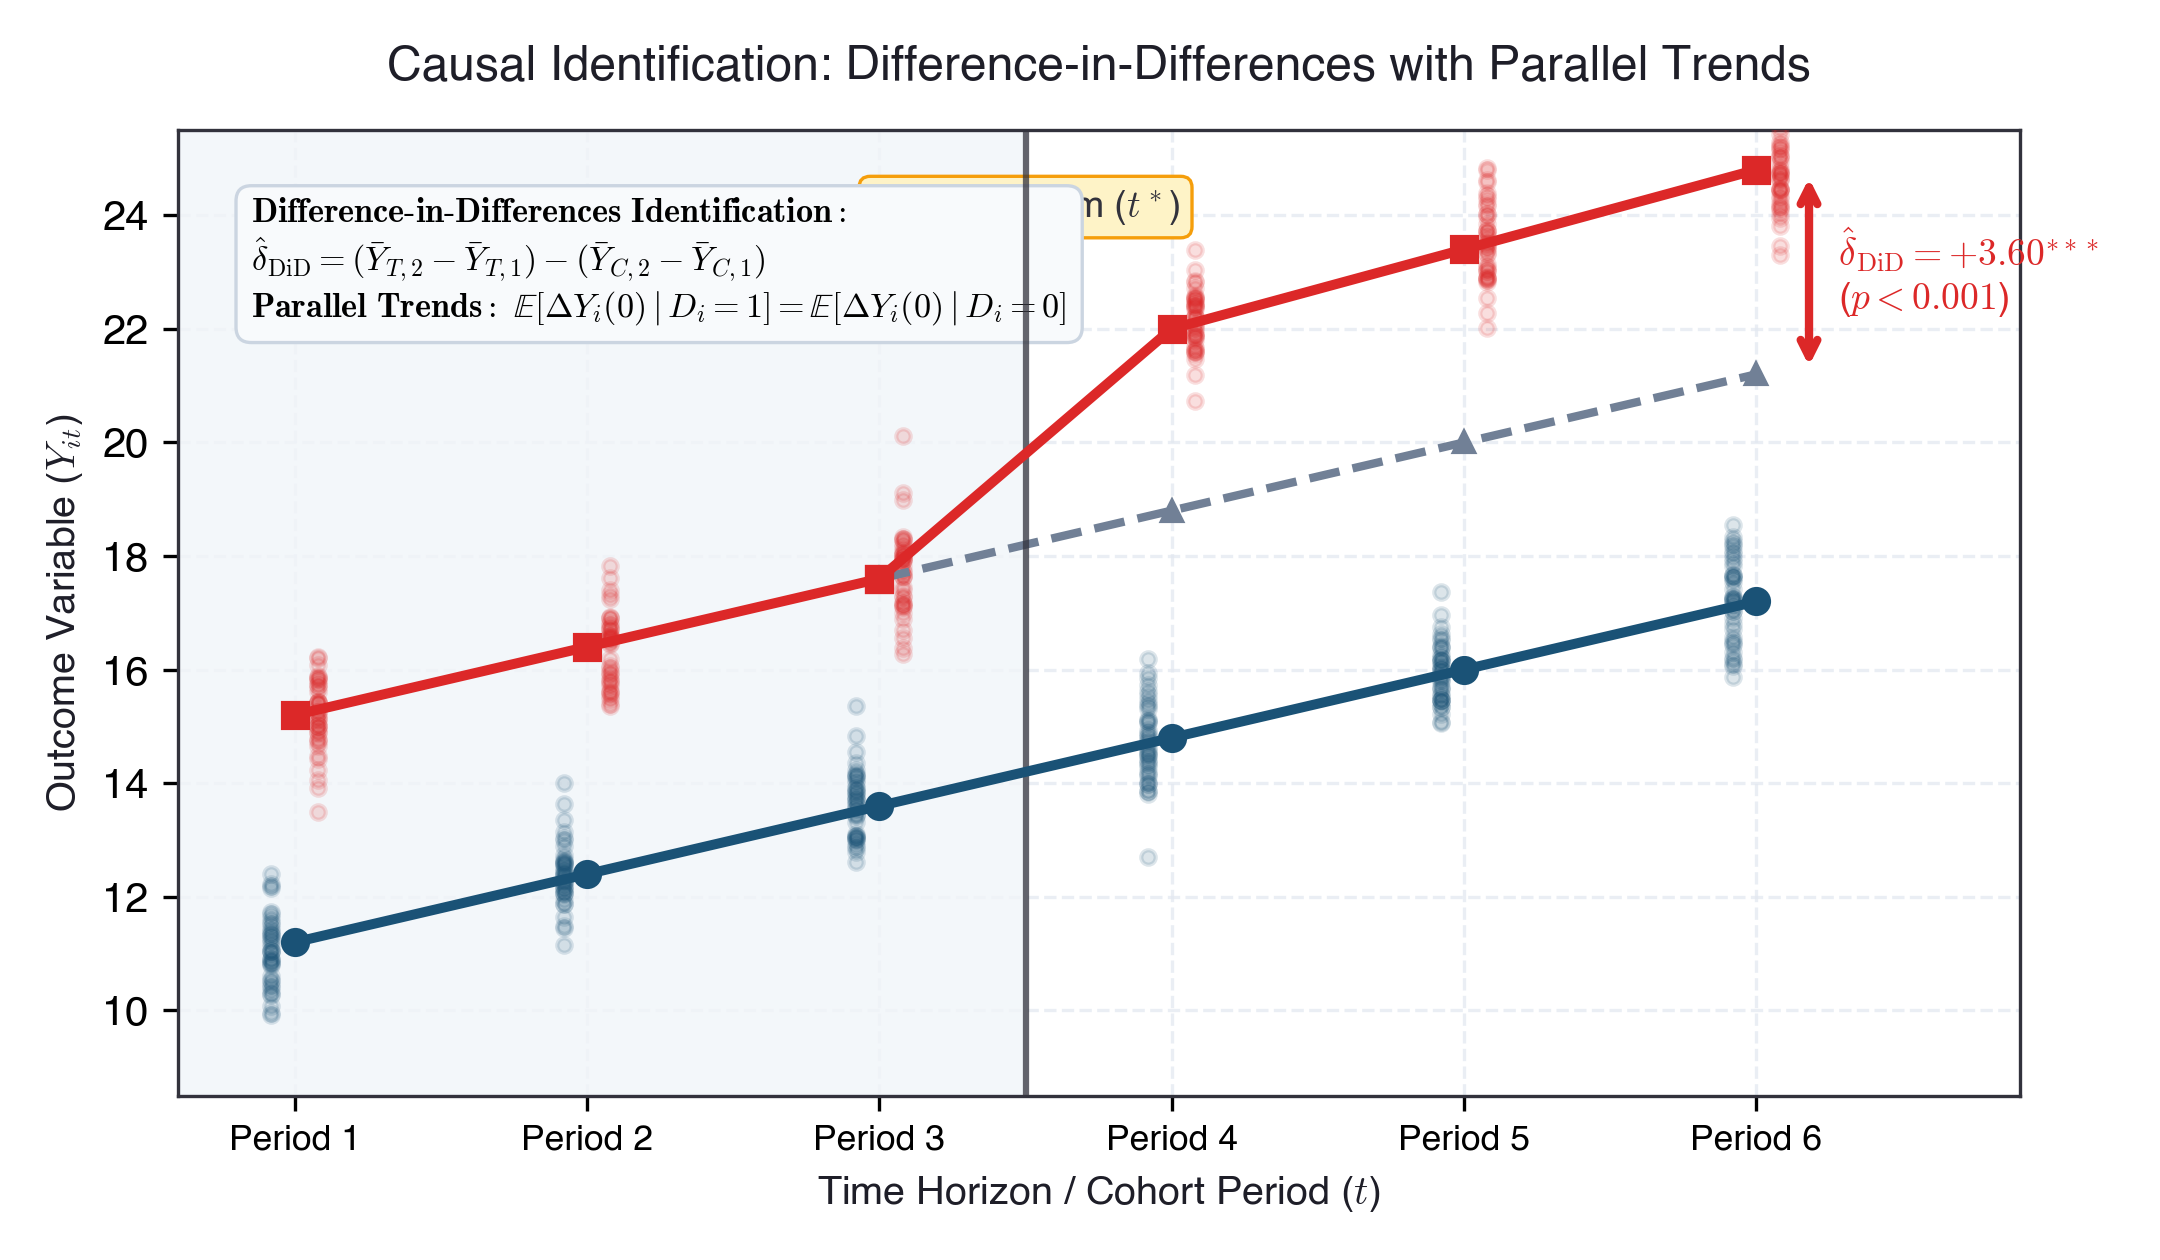
\includegraphics[width=\linewidth, height=0.68\textheight, keepaspectratio]{econometric_did_plot.png}\\[2pt]
            {\tiny\textcolor{structure!70}{Fig 1: High-DPI Python/SciPy DiD simulation with counterfactual path.}}
        \end{column}
    \end{columns}
\end{frame}

% --- Slide 5: Cluster-Robust Covariance ---
\section{Inference}
\begin{frame}{Cluster-Robust Inference: Liang-Zeger Estimator}
    \begin{columns}[t]
        \begin{column}{0.48\textwidth}
            \pillalt{AUTOCORRELATION PROBLEM}\par\vspace{0.2em}
            \scriptsize
            When errors $\varepsilon_{it}$ exhibit intra-cluster correlation across time:
            \begin{equation*}
                \mathbb{E}[\varepsilon_{ig} \varepsilon_{jg}' \mid \mathbf{X}] \neq \mathbf{0}
            \end{equation*}
            Standard default OLS standard errors underestimate variance by $40\text{--}70\%$, causing severe over-rejection of the null hypothesis.
        \end{column}
        \begin{column}{0.48\textwidth}
            \pill{SANDWICH COVARIANCE}\par\vspace{0.2em}
            \scriptsize
            Liang-Zeger Cluster-Robust Covariance Matrix:
            \begin{equation*}
                \widehat{\mathrm{Var}}_{\mathrm{CR}}(\hat{\boldsymbol{\beta}}) = (\mathbf{X}^\top \mathbf{X})^{-1} \left( \frac{G}{G-1} \frac{N-1}{N-K} \sum_{g=1}^G \mathbf{X}_g^\top \hat{\mathbf{e}}_g \hat{\mathbf{e}}_g^\top \mathbf{X}_g \right) (\mathbf{X}^\top \mathbf{X})^{-1}
            \end{equation*}
            \vspace{0.1em}
            \begin{takeaway}
                \textbf{Asymptotics:} Consistent as number of clusters $G \to \infty$.
            \end{takeaway}
        \end{column}
    \end{columns}
\end{frame}

% --- Slide 6: Publication-Grade Regression Table ---
\section{Results}
\begin{frame}{Multi-Specification Empirical Regression Results}
    \begin{columns}[c]
        \begin{column}{0.56\textwidth}
            \centering
            \setlength{\tabcolsep}{3.5pt}
            \scriptsize
            \begin{tabular}{@{} l c c c @{}}
                \toprule
                & \multicolumn{3}{c}{\textbf{Dependent Variable: Log Throughput ($Y_{it}$)}} \\
                \cmidrule(lr){2-4}
                \textbf{Regressor} & \textbf{(1) Pooled OLS} & \textbf{(2) Fixed Effects} & \textbf{(3) Dynamic 2SLS} \\
                \midrule
                $\mathrm{Treat} \times \mathrm{Post}$ ($\delta$) & $0.412^{***}$ & $0.384^{***}$ & $0.395^{***}$ \\
                                                                  & $(0.048)$     & $(0.032)$     & $(0.035)$     \\
                Covariate Factor ($\beta_1$)                     & $0.185^{**}$  & $0.142^{*}$   & $0.138^{*}$   \\
                                                                  & $(0.062)$     & $(0.055)$     & $(0.057)$     \\
                \midrule
                Unit Fixed Effects                                & No            & Yes           & Yes           \\
                Time Fixed Effects                                & No            & Yes           & Yes           \\
                $R^2$                                             & $0.742$       & $0.886$       & $0.879$       \\
                Observations                                      & $45{,}200$    & $45{,}200$    & $45{,}200$    \\
                \bottomrule
            \end{tabular}
            \par\vspace{2pt}
            {\tiny\textcolor{structure!70}{Cluster-robust standard errors in parentheses. $^{***}p<0.001$, $^{**}p<0.01$, $^{*}p<0.05$.}}
        \end{column}
        \begin{column}{0.42\textwidth}
            \pillalt{FINDINGS}\par\vspace{0.3em}
            \scriptsize
            \begin{itemize}\setlength{\itemsep}{2pt}
                \item \textbf{Causal Invariance:} Point estimate $\hat{\delta} \approx +0.39$ is robust across FE and 2SLS.
                \item \textbf{Precision:} Fixed effects reduce residual variance by $33\%$.
                \item \textbf{Specification:} Hausman test confirms endogeneity in pooled OLS ($p < 0.001$).
            \end{itemize}
        \end{column}
    \end{columns}
\end{frame}

% --- Slide 7: Python Code Listing ---
\begin{frame}[fragile]{Vectorized Cluster-Robust OLS in Python}
\begin{lstlisting}[language=Python, basicstyle=\ttfamily\scriptsize, keywordstyle=\color{accent}\bfseries, commentstyle=\color{structure!60}\itshape, stringstyle=\color{journalblue}, frame=single, rulecolor=\color{structure!20}, backgroundcolor=\color{structure!3}, numbers=left, numberstyle=\tiny\color{structure!50}]
import numpy as np

def estimate_twfe_robust(X: np.ndarray, y: np.ndarray, clusters: np.ndarray):
    """Vectorized OLS estimation with Liang-Zeger cluster-robust standard errors."""
    XtX_inv = np.linalg.inv(X.T @ X)
    beta_hat = XtX_inv @ (X.T @ y)
    residuals = y - (X @ beta_hat)
    
    unique_g = np.unique(clusters)
    G = len(unique_g)
    N, K = X.shape
    meat = np.zeros((K, K))
    for g in unique_g:
        idx = (clusters == g)
        X_g, e_g = X[idx], residuals[idx]
        meat += X_g.T @ np.outer(e_g, e_g) @ X_g
        
    df_adj = (G / (G - 1)) * ((N - 1) / (N - K))
    vcov_cr = df_adj * (XtX_inv @ meat @ XtX_inv)
    return beta_hat, np.sqrt(np.diagonal(vcov_cr))
\end{lstlisting}
\end{frame}

% --- Slide 8: Summary ---
\section{Summary}
\begin{frame}{Key Econometric Takeaways}
    \begin{columns}[t]
        \begin{column}{0.48\textwidth}
            \pill{SUMMARY}\par\vspace{0.3em}
            \begin{itemize}\setlength{\itemsep}{2.5pt}
                \item \textbf{Parallel Trends:} The cornerstone of Difference-in-Differences identification.
                \item \textbf{Fixed Effects:} Essential for unobserved confounder absorption.
                \item \textbf{Inference:} Always cluster standard errors at the level of treatment assignment.
            \end{itemize}
        \end{column}
        \begin{column}{0.48\textwidth}
            \pillalt{NEXT STEPS}\par\vspace{0.3em}
            \begin{itemize}\setlength{\itemsep}{2.5pt}
                \item \textbf{Problem Set 2:} Derive the asymptotic variance of 2SLS.
                \item \textbf{Lab 2:} Estimate event study DiD leads and lags in Python.
                \item \textbf{Office Hours:} Wednesday 14:00--16:00 (Econ Hall 210).
            \end{itemize}
            \vspace{0.3em}
            \begin{takeaway}
                \textbf{Contact:} \texttt{econ-instructor@university.edu}
            \end{takeaway}
        \end{column}
    \end{columns}
\end{frame}

% --- Slide 9: References ---
\begin{frame}[allowframebreaks]{References}
    \printbibliography
\end{frame}

\end{document}
